\documentclass[a4paper,12pt]{article} 
\usepackage{geometry}
\usepackage{wrapfig}
\geometry{
	a4paper,
	total={170mm,257mm},
	left=10mm,
	right=10mm,
	top=20mm,
}
\usepackage{titlesec}
\titlelabel{\thetitle.\quad} %точка в section

%%% Работа с русским языком
\usepackage{cmap}                           % поиск в PDF
\usepackage{mathtext} 			 	       % русские буквы в формулах
\usepackage[T2A]{fontenc}               % кодировка
\usepackage[utf8]{inputenc}              % кодировка исходного текста
\usepackage[english,russian]{babel}  % локализация и переносы

%Математика
\usepackage{amsmath,amsfonts,amssymb,amsthm,mathtools} % AMS
\usepackage{icomma} % "Умная" запятая

%% Шрифты
\usepackage{euscript}	 % Шрифт Евклид
\usepackage{mathrsfs} % Красивый матшрифт

\usepackage{gensymb}
\usepackage{graphicx}

\usepackage{mathtext} 
\usepackage{setspace}
\usepackage{tabularx}
\usepackage{longtable}
\usepackage{icomma}
\usepackage{euscript}
\usepackage{float}
\usepackage{cutwin}
\usepackage{mathrsfs}
\usepackage{adjustbox}
\usepackage{dashbox}
\usepackage[normalem]{ulem}	
\usepackage[babel=true]{microtype}
\RequirePackage[T1]{fontenc}
\usepackage{amsmath,amsfonts,amssymb,amsthm,mathrsfs,mathtools} 
\usepackage{xcolor}         
\usepackage{enumitem}     
\usepackage{xpatch}       
\usepackage{cancel}                  
\usepackage{upgreek}                 
\usepackage{lipsum}                  
\usepackage[version=4]{mhchem}       
\usepackage{multirow}                
\usepackage{stackengine}             
\usepackage{tikz}         
\usepackage{hyperref}
\hypersetup{colorlinks=true,urlcolor=blue}       
\usetikzlibrary{positioning}         
\usepackage{titletoc}                 
\usepackage{chngcntr}              
\usepackage{fancyhdr}                
\usepackage{makecell}                
\usepackage{indentfirst}             
\usepackage{tocloft}                 
\usepackage{soul}                   
\usepackage[stable]{footmisc}       
\usepackage{subfig}  
\usepackage{comment}                  


\mathtoolsset{showonlyrefs=true}


\theoremstyle{definition}
\newtheorem*{definition}{Определение}
\newtheorem{statement}{Предложение}[section]
\newtheorem{lemma}{Лемма}[section]
\newtheorem{theorem}{Теорема}[section]
\newtheorem*{theoremn}{Теорема}
\newtheorem*{corollary}{Следствие}
\newtheorem*{example}{Пример}
\newtheorem*{note}{Замечание}
\newtheorem*{problem}{Задача}


\counterwithout{footnote}{section}\DeclareRobustCommand{\divby}{%
	\mathrel{\text{\vbox{\baselineskip.65ex\lineskiplimit0pt\hbox{.}\hbox{.}\hbox{.}}}}%
}

\newcommand{\dotpr}[2]{\bra{#1}\ket{#2}}
\let\AA\relax
\let\emptyset\varnothing
\DeclareMathOperator*{\esssup}{ess sup}
\DeclareMathOperator*{\ord}{ord}
\DeclareMathOperator*{\supp}{supp}
\DeclareMathOperator*{\pr}{pr}
\DeclareMathOperator*{\Ker}{Ker}
\DeclareMathOperator*{\Vol}{Vol}
\DeclareMathOperator*{\rg}{rk}
\DeclareMathOperator*{\Ima}{Im}
\DeclareMathOperator*{\Alt}{Alt}
\DeclareMathOperator*{\Sym}{Sym}
\newcommand{\eqdef}{\stackrel{\text{\tiny{def}}}{=}}
\newcommand{\pp}{\partial}
\newcommand{\AA}{\mathcal{A}}
\newcommand{\BB}{\mathcal{B}}
\newcommand{\MM}{\mathbb{M}}
\newcommand{\NN}{\mathbb{N}}
\newcommand{\ZZ}{\mathbb{Z}}
\newcommand{\QQ}{\mathbb{Q}}
\newcommand{\RR}{\mathbb{R}}
\newcommand{\CC}{\mathbb{C}}
\newcommand{\FFF}{\mathbb{F}}
\newcommand{\DD}{\mathcal{D}}
\newcommand{\FF}{\mathcal{F}}
\newcommand{\sS}{\mathcal{S}}
\newcommand*\circled[1]{\tikz[baseline=(char.base)]{
		\node[shape=circle,draw,inner sep=2pt] (char) {#1};}}

%%% Заголовок
\author{Пазов Тенгиз, Симухин Егор Б03-302}
\title{Лабораторная работа 3.7.3 \\
	\textbf{Изучение длинной линии}}
\date{\today}

\begin{document}
	
{\Large \maketitle}

	\paragraph*{Цель работы:} ознакомится и проверить на практике теорию распространения
	электрических сигналов вдоль длинной линии; измерить амплитудо- и фазово-частотные
	характеристики коаксиальной линии; определить погонные характеристики такой
	линии; на примере модели длинной линии изучить вопрос распределения амплитуды
	колебаний сигнала по длине линии.
	\paragraph*{В работе используются:} осциллограф АКТАКОМ ADS-6142H; генератора АКИП 3420/1; бухта с коаксиальным кабелем pk 50-4-11; 
	схематический блок "модель длинной линии"; магазин сопротивления Р33, соединительные провода.

	\section{Введение}
	В данной работе сигналы передаются по длинному коаксиальному кабелю, который представляет из себя систему двух проводников -- изолированный коаксиальный медный проводящий цилиндр радиуса $r_2$ и тонкий медный проводник, имеющий радиус $r_1$ и расположенный на оси цилиндра. Пространство между ними заполнено веществом, имеющим диэлектрическую проницаемость $\varepsilon$ и магнитную восприимчивость $\mu$.
	
	\begin{figure}[h!]
		\centering
		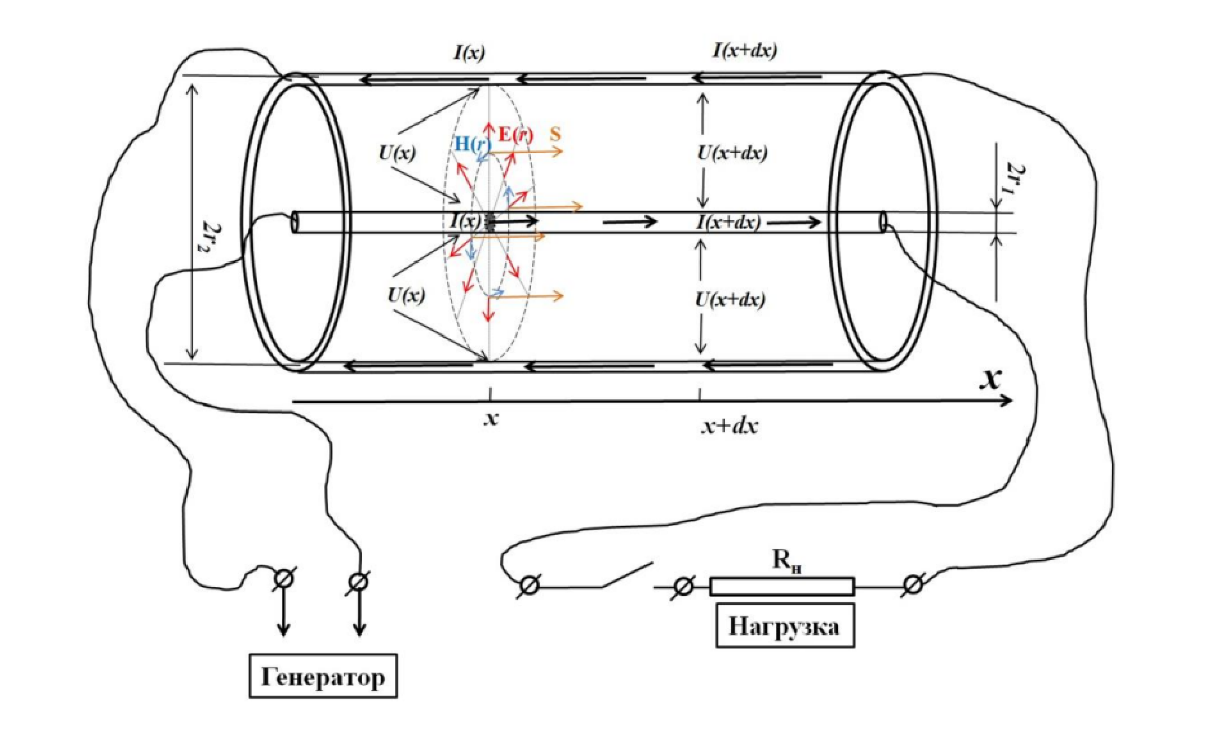
\includegraphics[scale=0.6]{1.png}
		\caption{Схема коаксиального кабеля}
	\end{figure}	
	Рассмотрим элемент $dx$ такого кабеля. Такой элемент обладает индуктивностью.
	\begin{equation}
		dL=2\mu\ln\left(\frac{r_2}{r_1}\right)dx
	\end{equation}
	величина $L_x=dL/dx=2\mu\ln\left(r_2/r_1\right)$ называется погонной индуктивностью.
	
	Так же два проводника обладают взаимной ёмкостью
	\begin{equation}
		dC=\frac{\varepsilon}{2\ln(r_2/r_1)}dx
	\end{equation}
	аналогично определяется погонная ёмкость $C_x=dC/dx=\frac{\varepsilon}{2\ln(r_2/r_1)}$. При передаче сигналов по такому кабелю возникают противоположно направленные токи по внешней оболочке и внутреннему проводнику, а также напряжение между проводниками. При высоких частотах величины $I$ и $U$ будут зависеть от $x$.
	Падение напряжения на концах выбранного элемента связано с возникновением ЭДС индукции и омическим сопротивлением. От сюда получим
	\begin{equation}\label{Ueq}
		U(x+dx)-U(x)=-\frac{L_xdx}{c^2}\frac{\partial I}{\partial t}-R_xIdx     
	\end{equation}
 	где $R_x= dR/dx= (\sigma S)^{-1}$ -- погонное сопротивление, $\sigma$ -- удельная проводимость, $S=\pi r_1^2$ -- площадь поперечного сечения проводника.
 	
 	Изменение силы тока связано с перетеканием части заряда на ёмкость, т.е
 	\begin{equation}\label{Ieq}
 		I(x+dx)-I(x)=-\frac{\partial q}{\partial t}=-C_x dx \frac{\partial U}{\partial t}
 	\end{equation}
 	
 	Разделив уравнения \eqref{Ueq} и \eqref{Ieq} на $dx$ получим систему.
 	\begin{equation}
 		\begin{cases}
 			\frac{\partial U}{\partial x}=-\frac{L_x}{c^2}\frac{\partial I}{\partial t}-R_xI
 			\\
 			\frac{\partial I}{\partial x}=-C_x\frac{\partial U}{\partial t}
 		\end{cases}
 	\end{equation}
 	Продифференцировав первое уравнение по $x$, а второе по $t$ получим
\begin{equation}\label{WaveSystUeq}
 		\begin{cases}
 			\frac{\partial^2 U}{\partial x^2}=-\frac{L_x}{c^2}\frac{\partial I}{\partial x\partial t}-R_x\frac{\partial I}{\partial x}
 			\\
 			\frac{\partial I}{\partial t\partial x}=-C_x\frac{\partial^2 U}{\partial t^2}
 		\end{cases}
\end{equation}
 	Итого получим уравнение
\begin{equation}\label{WaveUeq}
 		\frac{\partial^2 U}{\partial t^2}-V^2_\text{ф}\frac{\partial^2 U}{\partial x^2}+\gamma\frac{\partial U}{\partial t}=0
\end{equation}
 	где $V_\text{ф}=\frac{c}{\sqrt{L_xC_x}}$ -- фазовая скорость, $\gamma=R_xC_xV^2_\text{ф}$ -- декремент затухания. Подставив погонные характеристики в выражение для фазовой скорости, заметим, что фазовая скорость совпадает со скоростью распространения электромагнитных волн в среде.
 	\begin{equation}
 		V_\text{ф}=\frac{c}{\sqrt{\varepsilon\mu}}
 	\end{equation}
 	
 	Решение уравнения \eqref{WaveUeq} ищется в виде
 	\begin{equation}\label{WaveUsol}
 		U(x,t)=U_0e^{-i\omega t}e^{(-\alpha+ik)x}
 	\end{equation}
 	Из первого уравнения системы \eqref{WaveSystUeq} получается сила тока
 	\begin{equation}
 		I(x,t)=U_0\frac{C_x\omega}{k+i\alpha}e^{-i\omega t}e^{(-\alpha+ik)x}
 	\end{equation}
 	Зная это, получим значение импеданса
 	\begin{equation}
 		Z(\omega,k)=\frac{U(x,t)}{I(x,t)}=\frac{k+i\alpha}{C_x\omega}
 	\end{equation}
 	В пределе малых затуханий $\alpha\ll\omega$
 	\begin{equation}
 		Z\approx\frac{k}{C_x\omega}=\frac{1}{C_xV_\text{ф}}=\frac{1}{c}\sqrt{\frac{L_x}{C_x}}
 	\end{equation}
 	Если в конце замкнуть длинную линию на сопротивление $R_0=Z$, то отражённой волны не возникнет, т.к с точки зрения волны это будет эквивалентным продолжением линии. Иначе возникает отражённая волна, описываемая выражением
 	\begin{equation}
 		U(x,t)=U_0e^{-i\omega t}e^{-(\alpha+ik)x}
 	\end{equation}
 
 	Подстановка \eqref{WaveUsol} в \eqref{WaveUeq} даёт характеристическое уравнение
 	\begin{equation}
 		-\omega^2-V_\text{ф}^2(ki-\alpha)^2-i\omega\gamma=0
 	\end{equation}
 	От сюда получим систему
 	\begin{equation}
 		\begin{cases}
 			\omega^2=V_\text{ф}^2(k^2-\alpha^2)
 			\\
 			2\alpha kV_\text{ф}^2=\omega\gamma
 		\end{cases}
 	\end{equation}
 	Решая которую в пределе малых затуханий, получим
 	\begin{equation}\label{alphaSol}
 		\alpha=\frac{\omega}{V_\text{ф}}\sqrt{\frac{\sqrt{1+(\gamma/\omega)^2}-1}{2}}\approx\frac{\omega}{V_\text{ф}}\sqrt{\frac{\gamma^2}{4\omega^2}}=\frac{\gamma}{2V_\text{ф}}=R_xC_x\frac{V_\text{ф}}{2}
 	\end{equation}
 	\begin{equation}\label{kSol}
 		k=\frac{\omega}{V_\text{ф}}
 	\end{equation}
 	
 	Таким образом амплитуда напряжения на нагрузке будет иметь вид:
 	\begin{equation}\label{Un}
 		U_\text{н}(t)=U_0e^{-\alpha l}e^{ikl}e^{-\omega t}
 	\end{equation}
 	При этом амплитуда колебаний на согласованной нагрузке (в конце длинной линии) имеет вид:
 	\begin{equation}\label{UnAmp}
 		U_\text{н}=U_0e^{-\alpha l}
 	\end{equation}
 	Так же получена разность фаз
 	\begin{equation}\label{dphi}
 		\Delta \varphi=kl
 	\end{equation}
 	
 	Из уравнений \eqref{UnAmp} и \eqref{dphi} получим соотношения для экспериментального определения $\alpha$ и $k$ для различных $\omega$
 	\begin{equation}\label{alphaomega}
 		\alpha(\omega)=\frac{1}{l}\ln\frac{U_0}{U_\text{н}}
 	\end{equation}
 	\begin{equation}\label{komega}
 		k(\omega)=\frac{\Delta \varphi}{l}
 	\end{equation}

 	\subsection*{Экспериментальная установка}
 	Коаксиальный кабель подключается к генератору и осциллографу. На канал 1 выводится сигнал, подаваемый генератором, а с канала 2 снимается напряжение на нагрузке. Схема экспериментальной установки изображена ниже.
 	\newpage
 	\begin{figure}[h!]
 		\centering
 		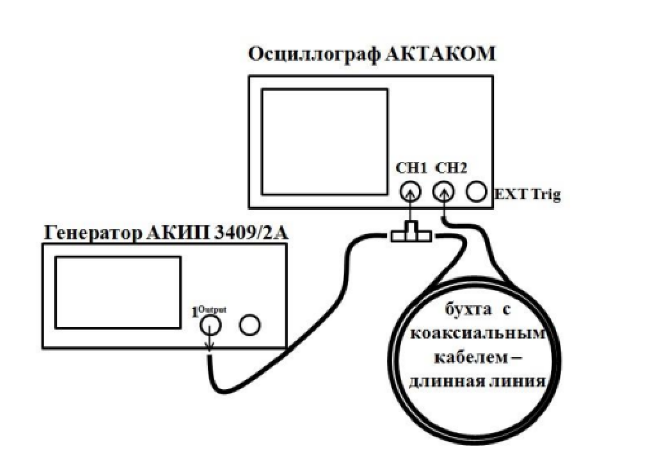
\includegraphics[scale=0.7]{2.png}
 		\caption{Схема экспериментальной установке}
 	\end{figure}
 
\section*{Ход работы}
	В данной работе кабель имеет длину $l=50,1$ м, $d = 1.3$ мм, $D = 4.0$ мм.
 	

\section{Оценка фазовой скорости}

	Снимем зависимости $U_0$, $U_H$, $\Delta \varphi$ от $\nu$. 
	Посчитаем $\omega$, $\alpha(\omega)$ и $k(\omega)$, 
	воспользовавшись формулами (8).

	\begin{table}[h]
		\centering
		\begin{tabular}{|l|l|l|l|} \hline
			$\nu$, МГц 
					& $U_{0}$, В 
						   & $U_{H}$, В 
								  & $\Delta \varphi$  \\ \hline
			1       & 17,40 & 15,80 &  1,57\\ \hline
			3       & 17,40 & 15,80 &  4,73\\ \hline
			5       & 17,40 & 15,20 & 7,88\\ \hline
			7       & 17,40 & 14,80 & 11,03\\ \hline
			9       & 17,40 & 14,20 & 14,19\\ \hline
			11      & 17,40 & 14,20 & 17,34\\ \hline
			13      & 17,40 & 14,00 & 20,50\\ \hline
			15      & 17,40 & 14,00 & 23,65\\ \hline
			17      & 17,40 & 13,60 & 26,81\\ \hline
			19      & 17,40 & 13,60 & 26,96\\ \hline
			21      & 17,40 & 13,00 & 33,11\\ \hline
			23      & 17,40 & 13,00 & 36,27\\ \hline
			25      & 17,40 & 12,80 & 39,42\\ \hline
			27      & 17,40 & 12,60 & 42,58\\ \hline
			29      & 17,40 & 12,60 & 45,73\\
            \hline
			31      & 17,40 & 11,80 & 48,89\\
            \hline
			33      & 17,40 & 11,80 & 52,04\\ 
            \hline
			35      & 17,40 & 11,40 & 55,19\\ 
            \hline
			37      & 17,40 & 11,40 & 58,35\\ 
            \hline
			39      & 17,40 & 11,00 & 61,5\\ 
            \hline
		\end{tabular}
	\end{table}
Для определения характеристик коаксиального кабеля  первое уравнение системы (22) с учетом (23) удобно переписать следующим образом:
\begin{equation}
    y = \frac{L_{x}C_{x}}{c^{2}}x
\end{equation}
где x = $\omega^{2}$, y = $k(\omega)^{2} - \alpha(\omega)^{2}$
По коэффициенту наклона данного графика установим произведение $L_{x}C_{x}$ и зная волновое сопротивление коаксиального кабеля c учетом (20) определили погонные характеристики кабеля.}
 	\begin{figure}[h!]
 		\centering
 		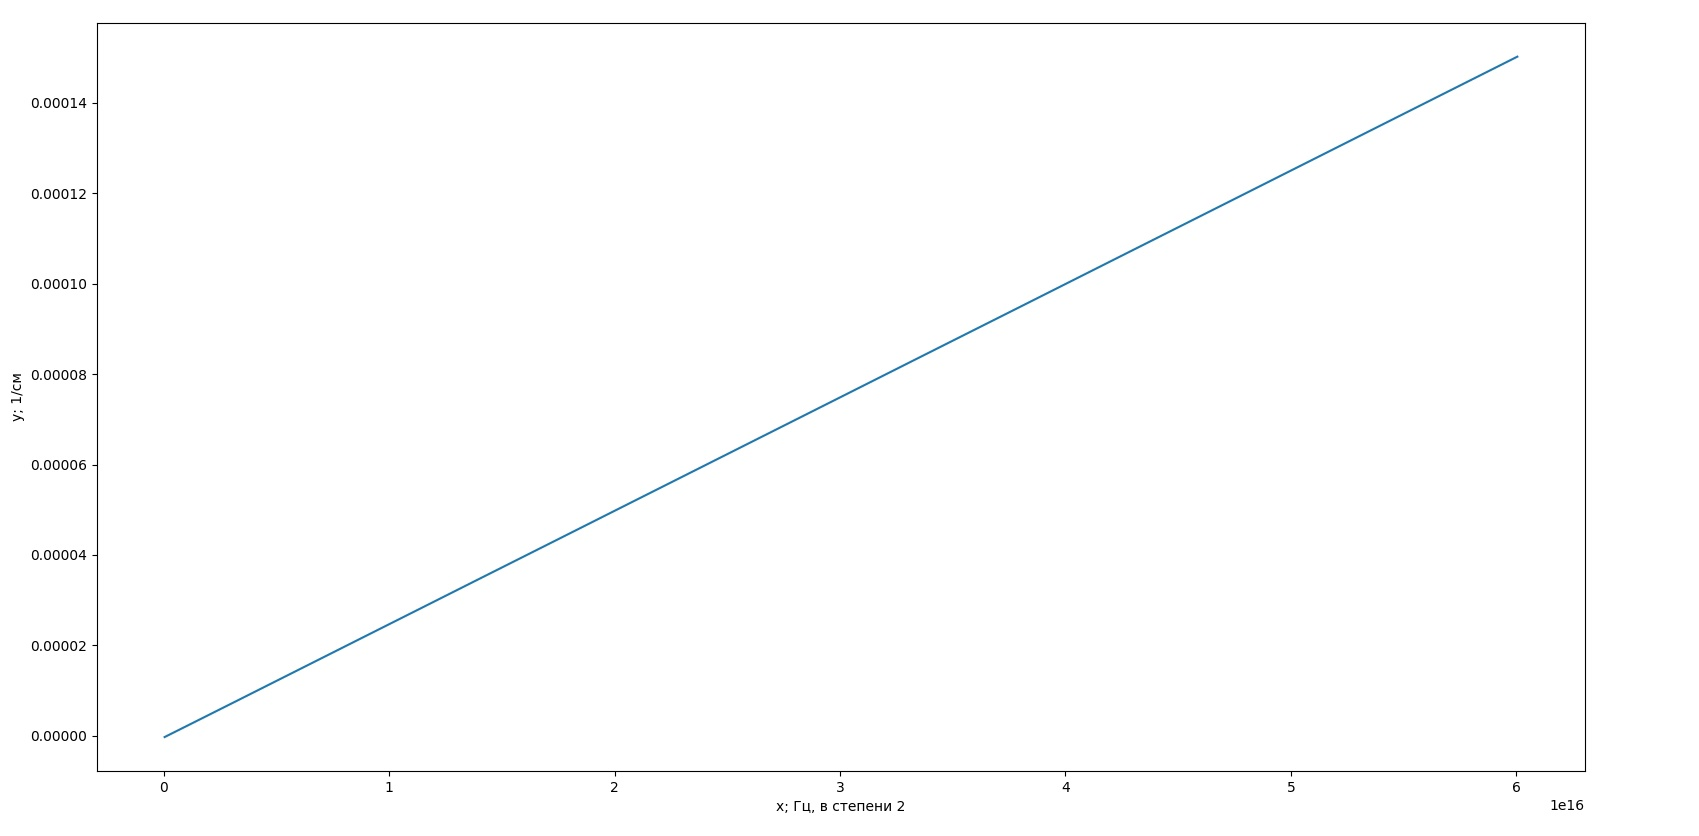
\includegraphics[scale=0.3]{3.jpg}
 		\caption{y1(x1)}
 	\end{figure}
	Результаты измерений резонансных частот приведены выше. По этим данным построим график $y(x)$ и определим:
 \begin{equation}
    L_{x}C_{x} 
\end{equation}


	Полученный коэффициент наклона
 \begin{equation}
    L_{x}C_{x} = 2,25 cm^{2}
\end{equation}
	От куда получим погонные характеристики
	\begin{equation}
            L_{x} = 2,78 \text{ см }
            C_{x} = 0,81 \text{ см}
	\end{equation}
 Тогда $V_{\text{ф}} = \frac{c^{2}}{L_{x}C_{x}} = 19,9 \cdot 10^{10}$
Зная геометрические параметры коаксиального кабеля с помощью выражений (2) и (4) определили диэлектрическую проницаемостью $\varepsilon$ и магнитную восприимчивость $\mu$
\begin{equation}
    \varepsilon = 1,83 \pm 0,02 \text{ }
    \mu = 1,23 \pm 0,03
\end{equation}
материала, заполняющего пространство между проводниками в кабеле.

	\section{Определение удельной проводимости проводников}
	\subsection{Метод А}
	
	Имеем соотношение
	\begin{equation}
		\alpha = \frac{4}{\sqrt{\sigma} d}C_x\frac{V_\text{ф}}{c}\sqrt{\nu}+\alpha_0
	\end{equation}
	где $\alpha_0$ -- поправочный коэффициент. Построим зависимость $y_2(x_2)$, где $y_2=\alpha$, $x_2=\sqrt{\nu}$.
	
	Полученное значение коэффициента наклона
	\begin{equation}
		a=\frac{4}{\sqrt{\sigma} d}C_x\frac{V_\text{ф}}{c}=(1.38\pm0,07)\cdot10^{-8}\:\text{см}\cdot\text{c}^{1/2}
	\end{equation}

	Отсюда получим
	\begin{equation}
		\sigma_1 = \left(\frac{2C_xV_\text{ф}}{acd}\right)^2=(3,58\pm0.08)\cdot10^{17}\:\text{ед.СГС}
	\end{equation}
	
	\begin{figure}[h]
		\centering
		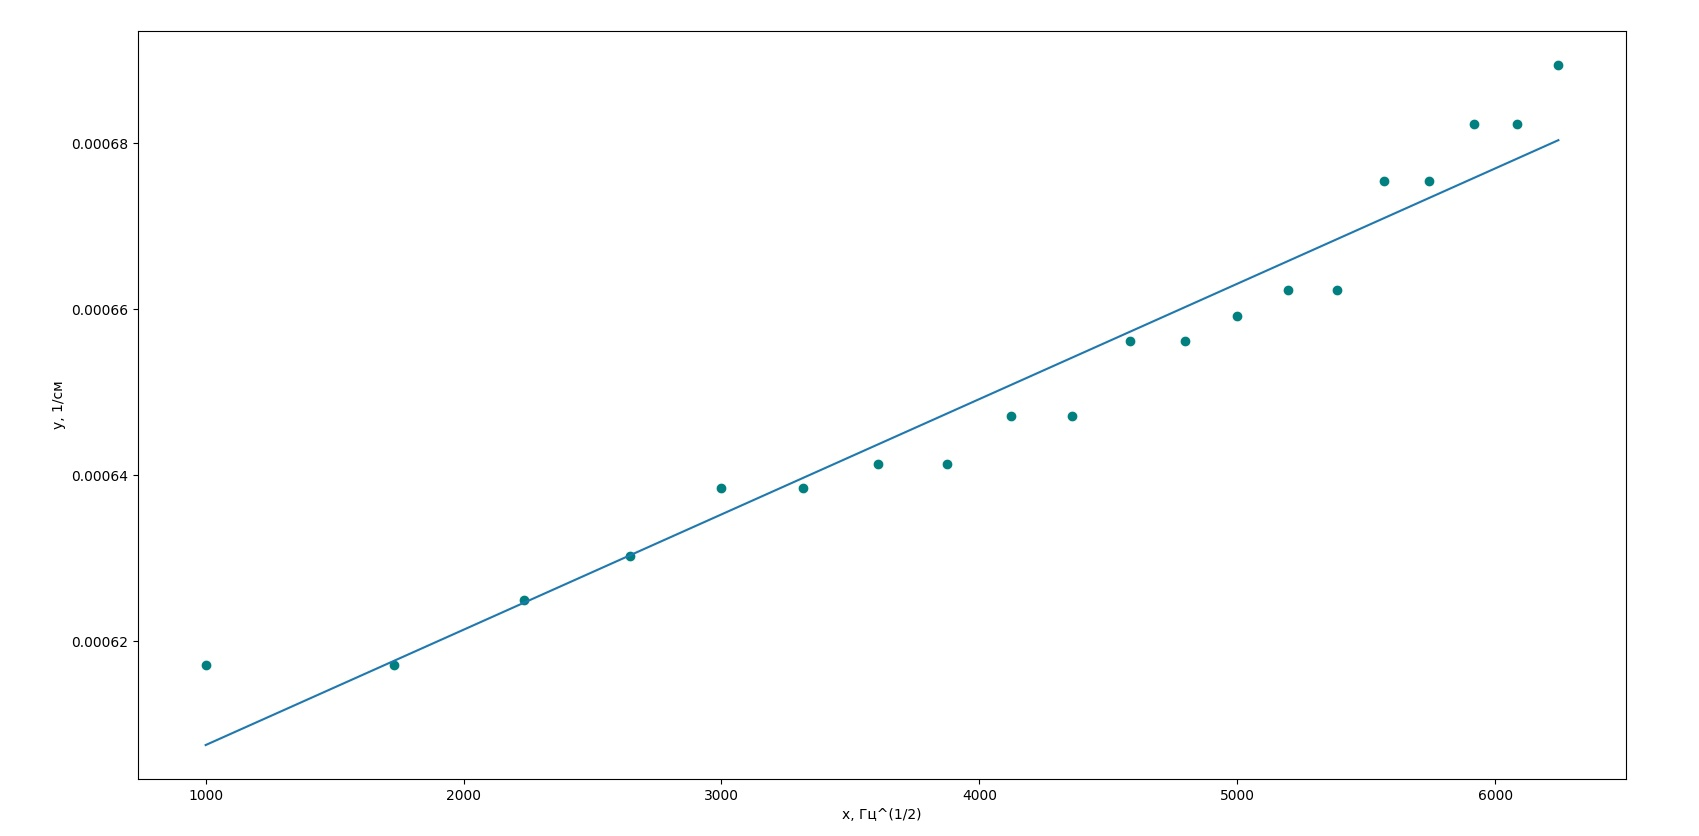
\includegraphics[scale=0.3]{4.jpg}
		\caption{График $y_2(x_2)$}
	\end{figure}
	
	\subsection{Метод Б}
	Из теории известно, что 
	\begin{equation}
		2\alpha k=\omega R_xC_x
	\end{equation}
	Которое можно свести к зависимости
	\begin{equation}
		y_3=\frac{4\pi C_x}{cd\sqrt{\sigma}}x_3
	\end{equation}
	где $x_3=\nu^{3/2}$, $y_3=a(\omega) \cdot k(\omega)$.
	\begin{figure}[h!]
		\centering
		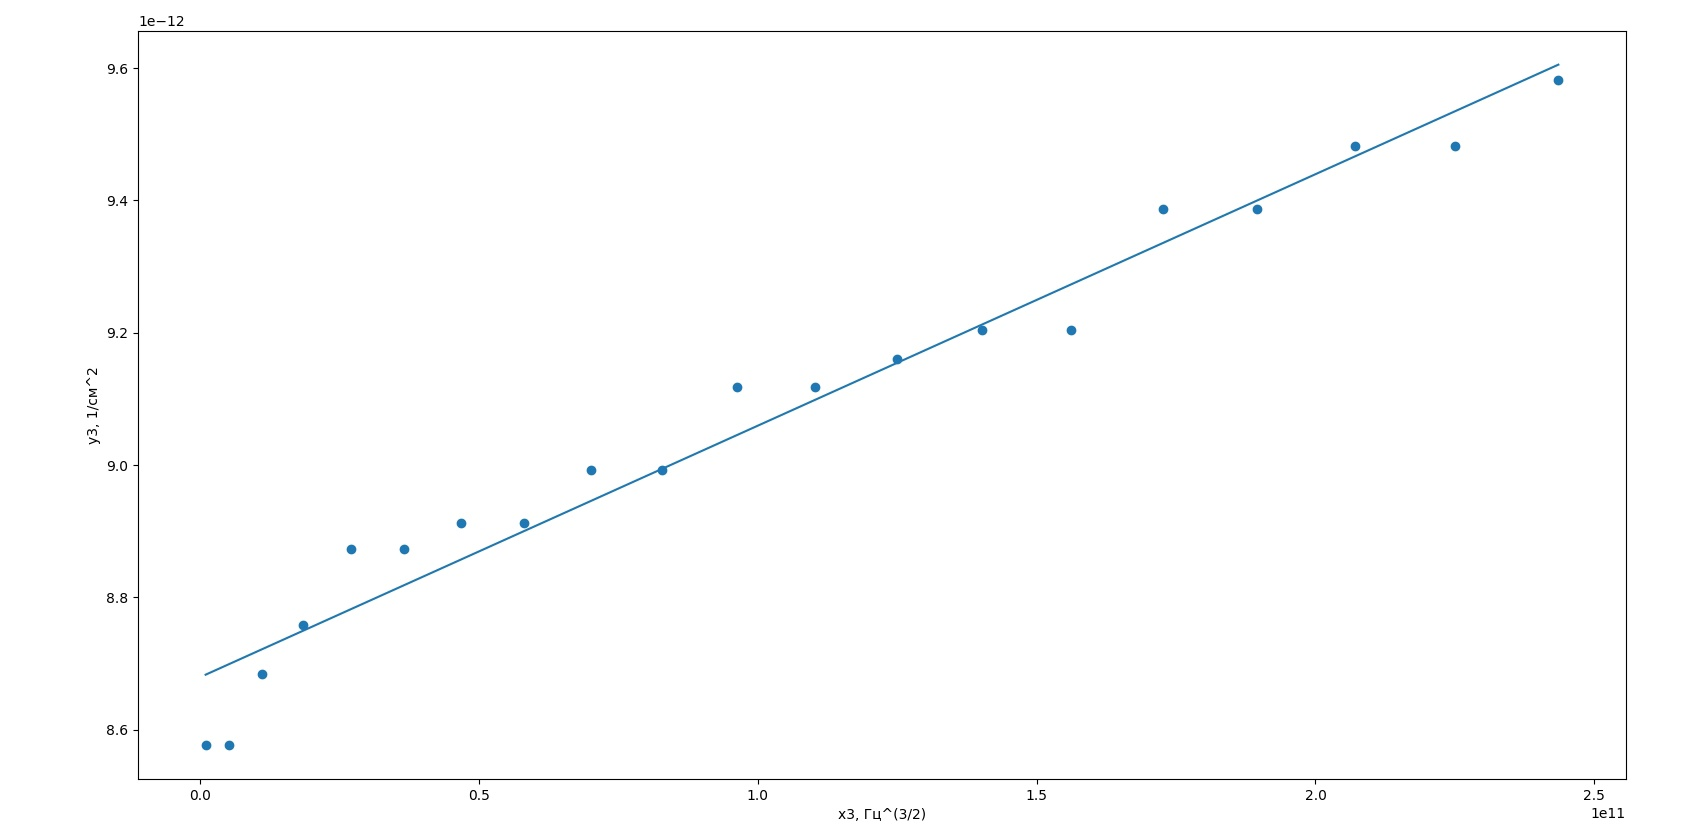
\includegraphics[scale=0.3]{5.jpg}
		\caption{График $y_3(x_3)$}
	\end{figure}

	Полученное значение коэффициента наклона
	\[a=\frac{4\pi C_x}{cd\sqrt{\sigma}}=(3.76\pm0.02)\cdot10^{-18}\:\text{ед.СГС}\]
	Отсюда получим
	\begin{equation}
		\sigma_2=\left(\frac{4\pi C_x}{acd}\right)^2=(4,74\pm0.05)\cdot10^{17}\:\text{ед.СГС}
	\end{equation}
\newpage
	\begin{figure}[h!]
		\centering
		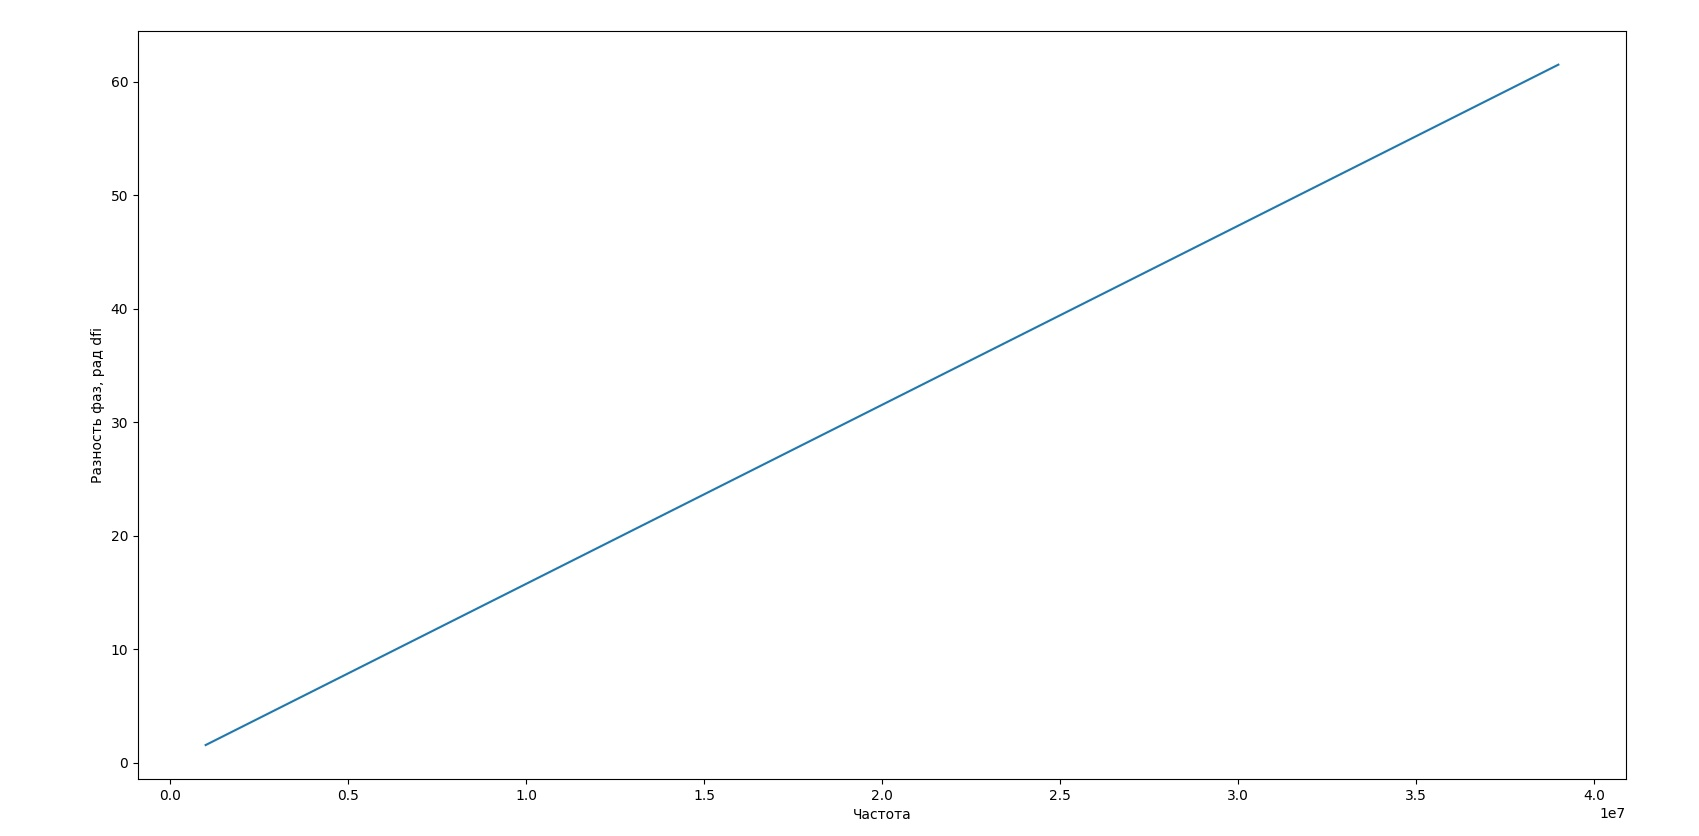
\includegraphics[scale=0.3]{6.jpg}
		\caption{ФЧХ}
	\end{figure}
	\section{Вывод}
 \begin{figure}[h!]
 		\centering
 		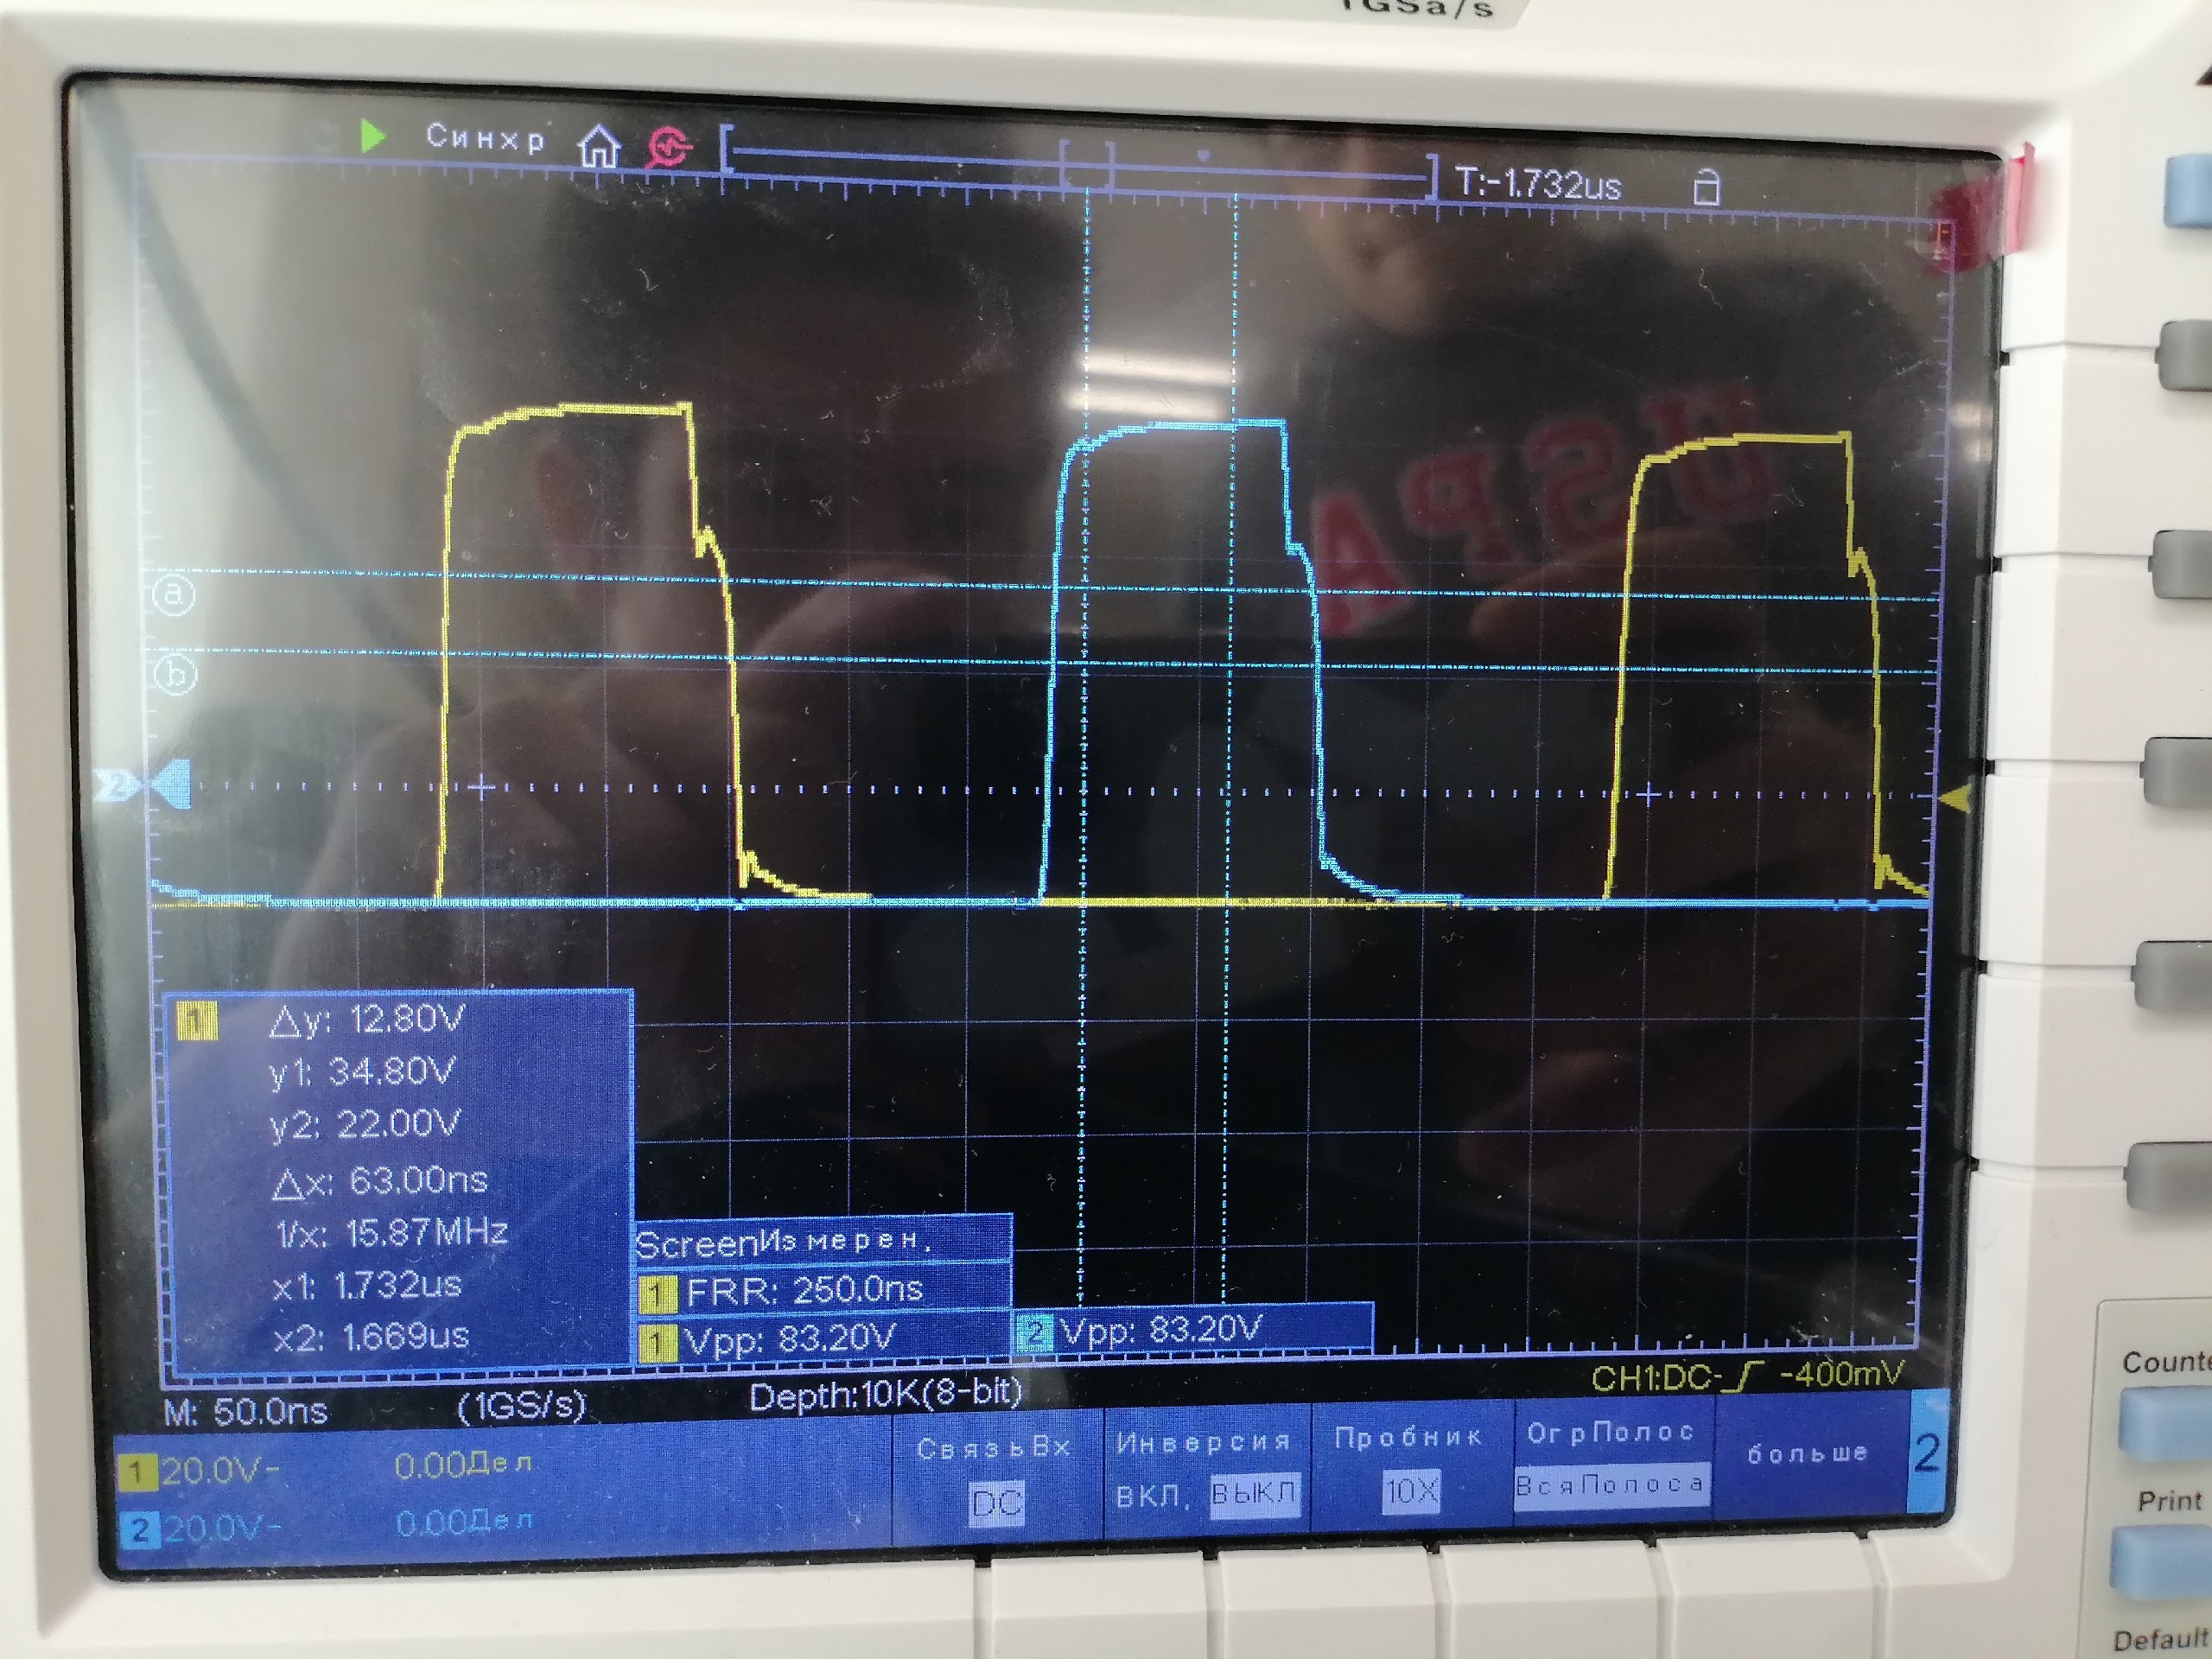
\includegraphics[scale=0.2]{7.jpg}
 		\caption{Нагрузка \Omega = 1MOm}
 	\end{figure}
  \begin{figure}[h!]
 		\centering
 		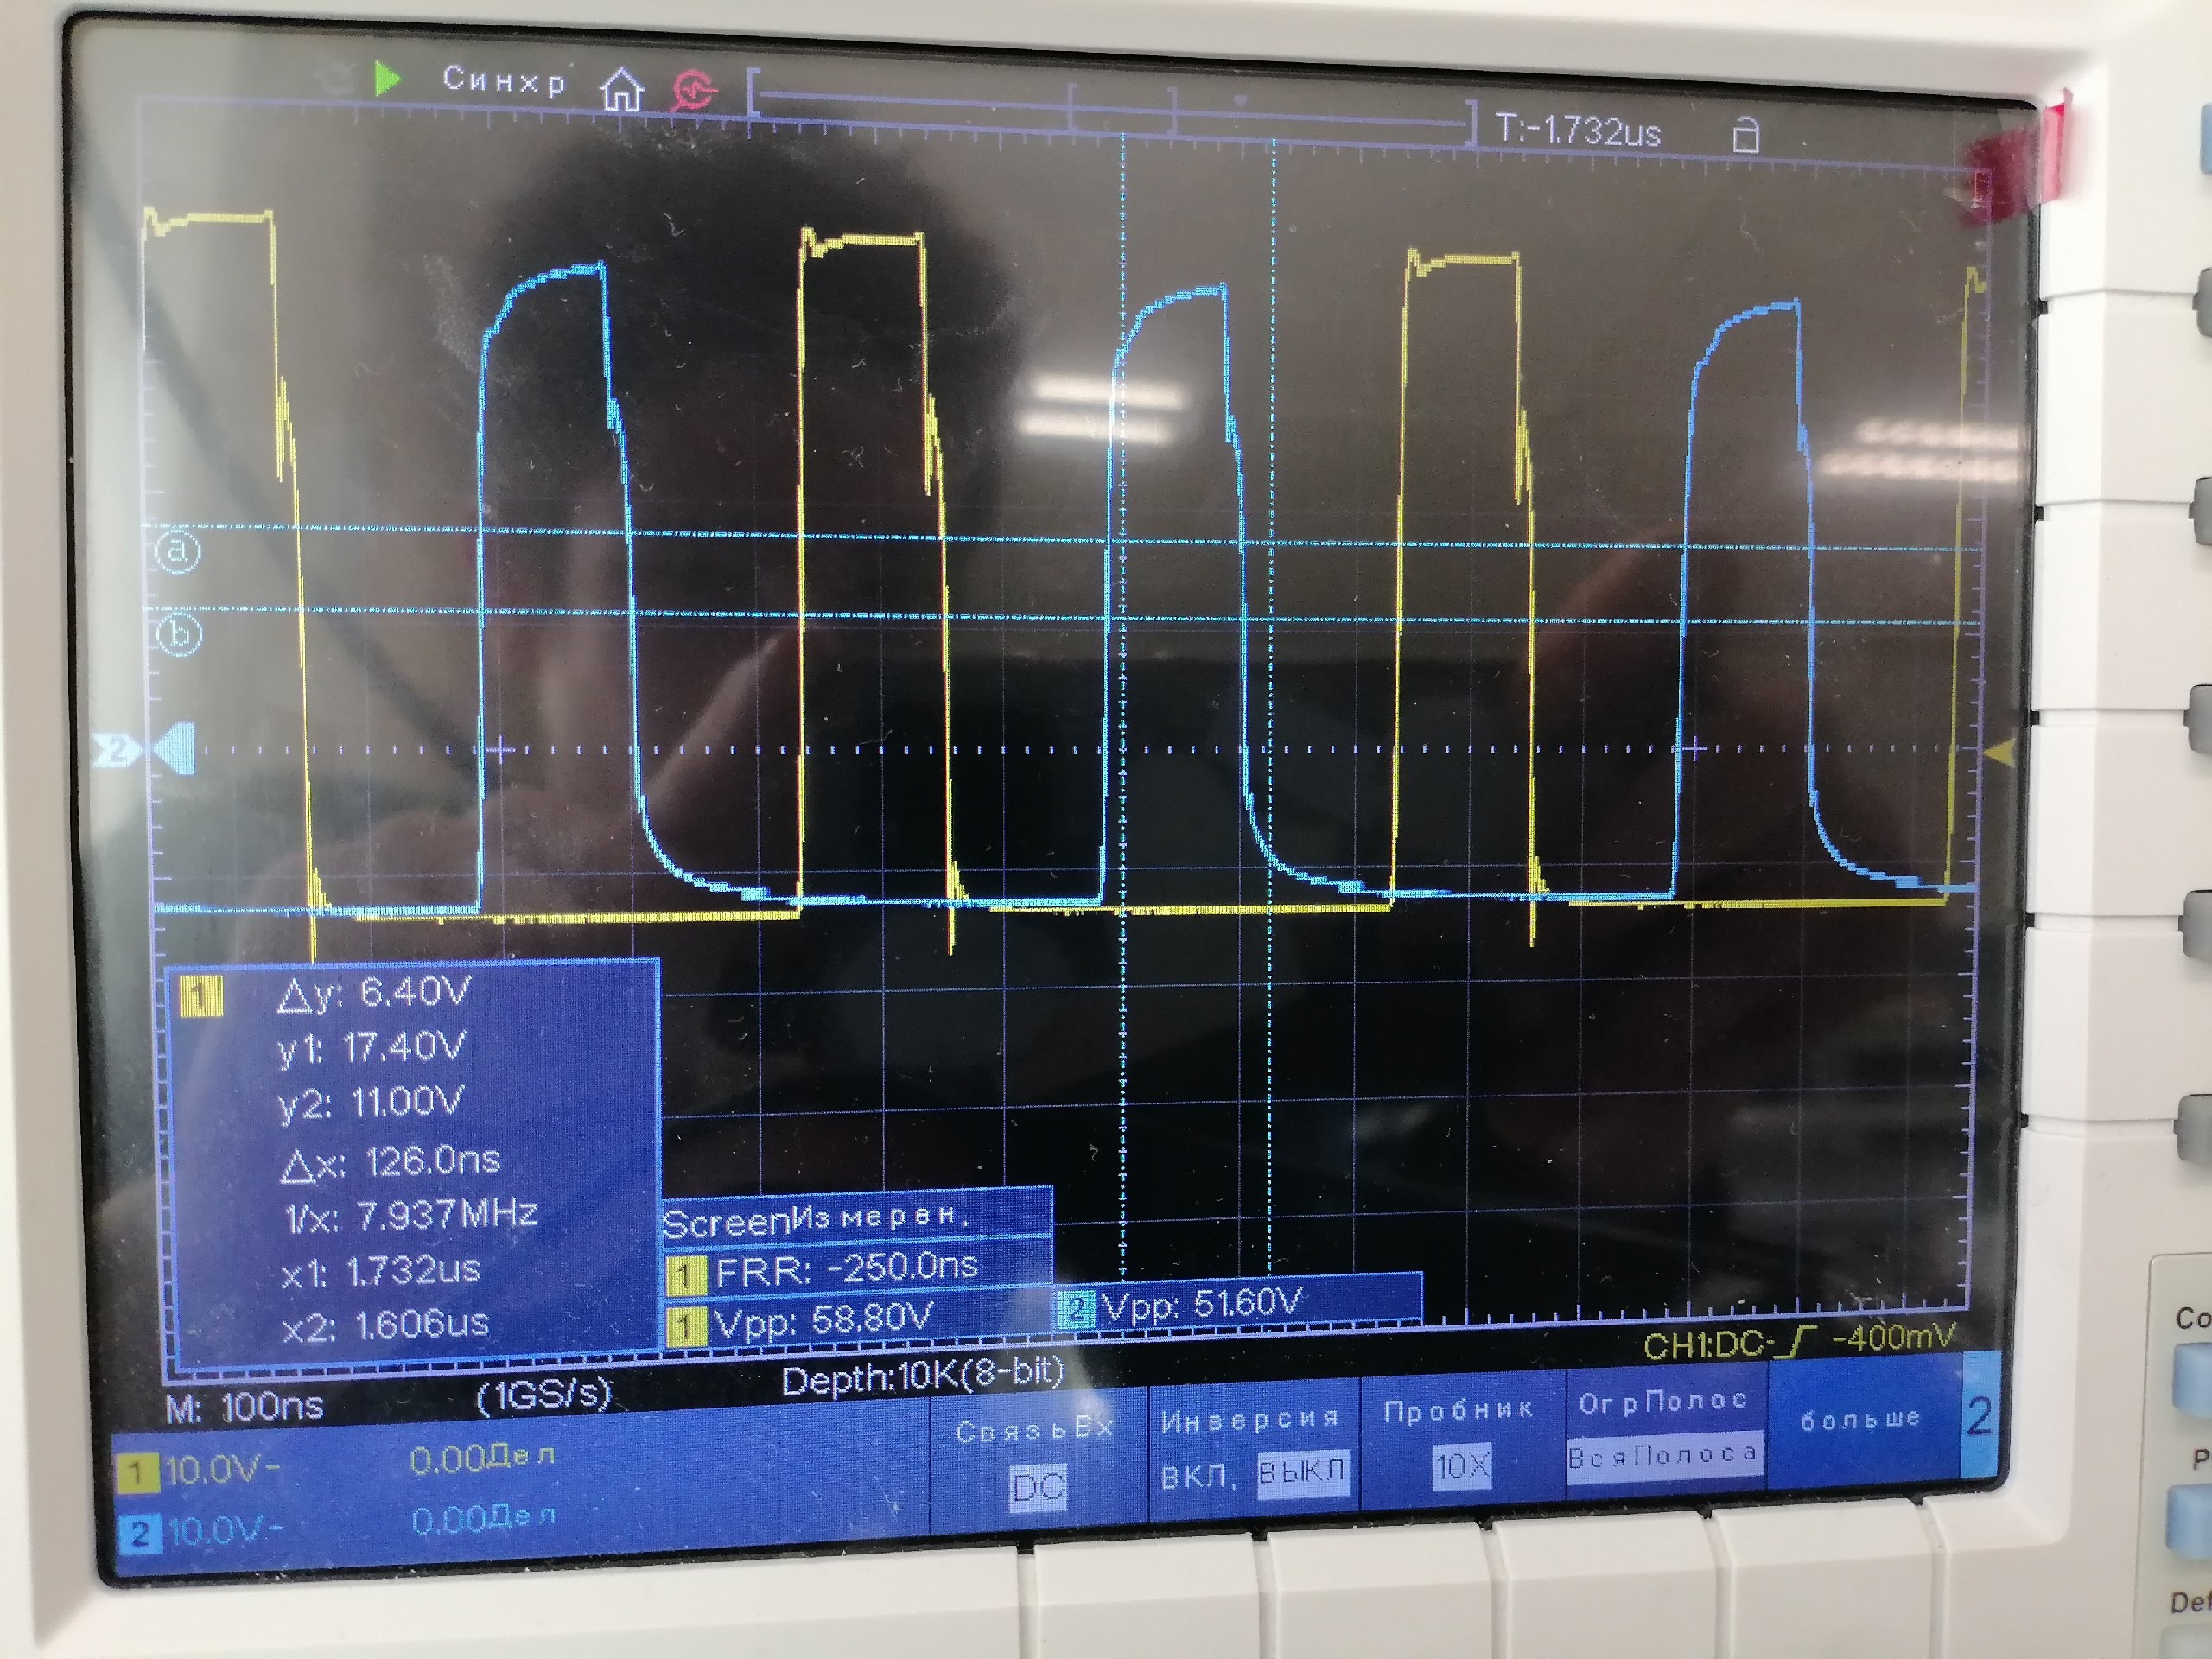
\includegraphics[scale=0.2]{8.jpg}
 		\caption{Согласованная нагрузка(меандр)}
 	\end{figure}
Проведя исследование длинной линии и изучив изменение электрического сигнала на ее концах, мы разработали способы определения фазовой скорости сигналов различных форм. Благодаря использованию амплитудно-частотной характеристики длинной линии, мы смогли определить ее характеристики, такие как диэлектрическая и магнитная проницаемости слоя между проводящими элементами. Преобразовав ФЧХ с помощью вспомогательных величин, таких как коэффициент затухания и волновой коэффициент, мы также изучили несколько способов определения удельной проводимости материала. Однако, результаты этих способов заметно отличались друг от друга.

\end{document}
